% Ejemplo de documento LaTeX
% Tipo de documento y tamaño de letra
\documentclass[10pt]{article}
% Preparando para documento en Español.
% Para documento en Inglés no hay que hacer esto.
\usepackage[spanish]{babel}
\selectlanguage{spanish}
\usepackage[utf8]{inputenc}


% EL titulo, autor y fecha del documento
\title{Graficando series de Taylor}
\author{Rios Quijada Danira}
\date{28 de Febrero de 2015}
% Aqui comienza el cuerpo del documento
\usepackage{graphicx}
\begin{document}
% Construye el título
\maketitle
\section{Teorema de Taylor}
En cálculo, el teorema de Taylor, recibe su nombre del matemático británico Brook Taylor, quien lo enunció en 1712. Este teorema permite obtener aproximaciones polinómicas de una función en un entorno de cierto punto en que la función sea diferenciable.

En esta actividad hicimos varias series de taylor, de distintos grados para distintas funciones, graficando los resultados. 

\section{sin(x)} 
\subsection{Código}
\begin{tabular}{l}
\begin{verbatim}  
 /* [wxMaxima batch file version 1] [ DO NOT EDIT BY HAND! ]*/
/* [ Created with wxMaxima version 13.04.2 ] */
/* [wxMaxima: input start ] */
f(x):=sin(x);
P1(x):=taylor(f(x), x, 0, 1);
P3(x):=taylor(f(x), x, 0, 3);
P5(x):=taylor(f(x), x, 0, 5);
P7(x):=taylor(f(x), x, 0, 7);
tex(P1(x));
tex(P3(x));
tex(P5(x));
tex(P7(x));
plot2d ([P1(x), P3(x), P5(x), P7(x), f(x)], [x, -%pi, %pi],
[color, blue, green, red, black, cyan], [legend, "f", "P1", 
"P3", "P5", "P7"],[axes, true], [xlabel, "x"],
[ylabel, "sin(x)"]);
/* [wxMaxima: input end ] */
/* Maxima can't load/batch files which end with a comment! */
"Created with wxMaxima"$
\end{verbatim} \\

\begin{figure}
  \centering
    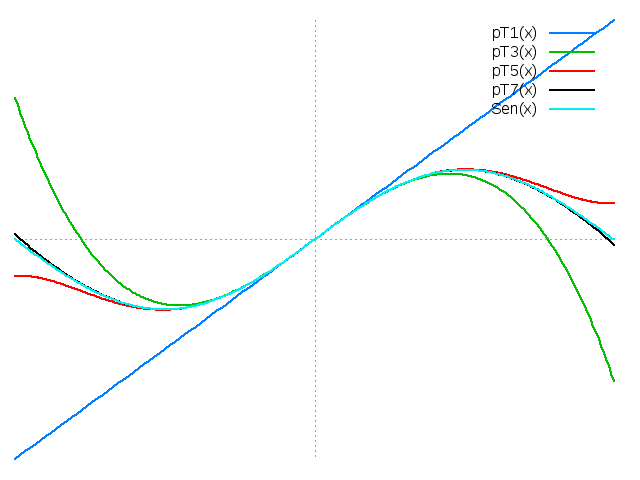
\includegraphics[scale=0.4]{sinx}
\end{figure}
\end{tabular}
\newpage 




\section{log (1+x)}



\subsection{Código}
\begin{tabular}{l}
\begin{verbatim}  
 /* [wxMaxima batch file version 1] [ DO NOT EDIT BY HAND! ]*/
/* [ Created with wxMaxima version 13.04.2 ] */
/* [wxMaxima: input start ] */
f(x):=log(1+x);
T4(x):=taylor(f(x), x, 0, 4);
T7(x):=taylor(f(x), x, 0, 7);
T11(x):=taylor(f(x), x, 0, 11);
T16(x):=taylor(f(x), x, 0, 16);
tex(T4(x));
tex(T7(x));
tex(T11(x));
tex(T16(x));
plot2d ([T4(x), T7(x), T11(x), T16(x), f(x)], [x, -1.5, 1.5], [y, -4,2],
[color, red, green, blue, cyan, orange],
[legend, "T4", "T7", "T11", "T16", "f"],[axes, true],
[xlabel,"x"], [ylabel, "log(1+x)"]);
/* [wxMaxima: input end ] */
/* Maxima can't load/batch files which end with a comment! */
"Created with wxMaxima"$
\end{verbatim} \\
\begin{figure}
  \centering
    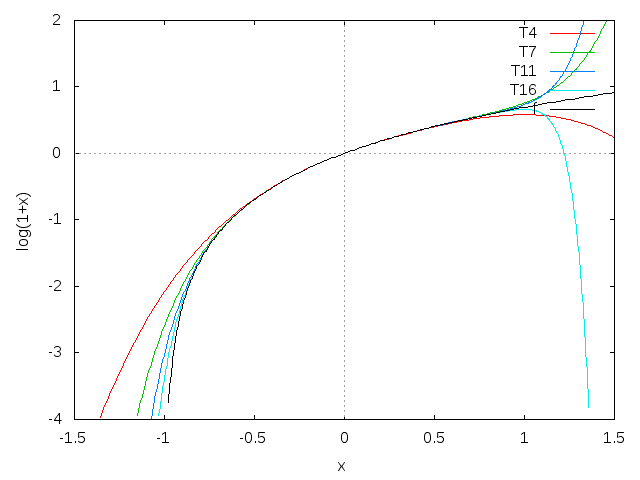
\includegraphics[scale=0.4]{log1}
\end{figure}
\end{tabular}



\newpage

\section{log(cos(x))}


\subsection{Código}
\begin{tabular}{l}
\begin{verbatim}  
  /* [wxMaxima batch file version 1] [ DO NOT EDIT BY HAND! ]*/
/* [ Created with wxMaxima version 13.04.2 ] */
/* [wxMaxima: input start ] */
f(x):=log(cos(x));
t3(x):=taylor(f(x), x, 0, 3);
t6(x):=taylor(f(x), x, 0, 6);
t9(x):=taylor(f(x), x, 0, 9);
t12(x):=taylor(f(x), x, 0, 12);
tex(t3(x));
tex(t6(x));
tex(t9(x));
tex(t12(x));
plot2d ([f(x), t3(x), t6(x), t9(x), t12(x)], [x, -0.5*%pi, 0.5*%pi], [y, -2,0.5],
[color, green, blue, red, cyan, orange],
[legend, "f", "t3", "t6", "t9", "t12"], [axes, true], [xlabel,"x"], 
[ylabel, "log(cos(x))"]);
/* [wxMaxima: input end ] */
/* Maxima can't load/batch files which end with a comment! */
"Created with wxMaxima"$
\end{verbatim} \\
\begin{figure}
  \centering
    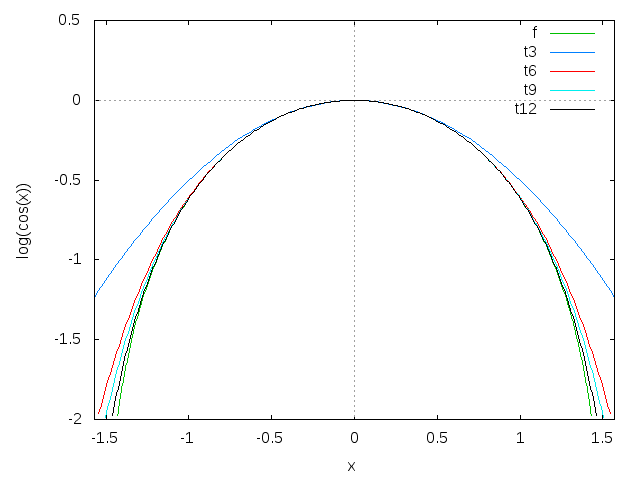
\includegraphics[scale=0.4]{logcos}
\end{figure}
\end{tabular}


\newpage


\section{exp(x)/cos(x)}


\subsection{Código}
\begin{tabular}{l}
\begin{verbatim}  
 /* [wxMaxima batch file version 1] [ DO NOT EDIT BY HAND! ]*/
/* [ Created with wxMaxima version 13.04.2 ] */
/* [wxMaxima: input start ] */
f(x):=exp(x)/cos(x);
p5(x):=taylor(f(x), x, 0, 5);
p10(x):=taylor(f(x), x, 0, 10);
p15(x):=taylor(f(x), x, 0, 15);
p20(x):=taylor(f(x), x, 0, 20);
tex(p5(x));
tex(p10(x));
tex(p15(x));
tex(p20(x));
plot2d ([f(x), p5(x), p10(x), p15(x), p20(x)], [x, -4, 4], [y, -3,10],
[color, blue, cyan, green, red, orange],
[legend, "f", "p5", "p10", "p15","p20"],
[axes, true], [xlabel,"x"], [ylabel, "exp(x)/cos(x)"]);
/* [wxMaxima: input end ] */
/* Maxima can't load/batch files which end with a comment! */
"Created with wxMaxima"$ 
\end{verbatim} \\
\begin{figure}
  \centering
    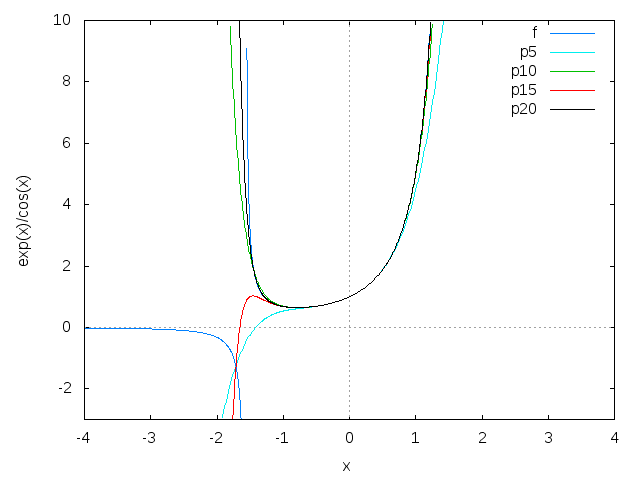
\includegraphics[scale=0.4]{expcos}
\end{figure}
\end{tabular}


\newpage


\section{(1+x)(exp(x))}


\subsection{Código}
\begin{tabular}{l}
\begin{verbatim}  
 /* [wxMaxima batch file version 1] [ DO NOT EDIT BY HAND! ]*/
/* [ Created with wxMaxima version 13.04.2 ] */
/* [wxMaxima: input start ] */
f(x):=(1+x)*exp(x);
t5(x):=taylor(f(x), x, 0, 5);
t10(x):=taylor(f(x), x, 0, 10);
t15(x):=taylor(f(x), x, 0, 15);
t20(x):=taylor(f(x), x, 0, 20);
tex(t5(x));
tex(t10(x));
tex(t15(x));
tex(t20(x));
plot2d ([t5(x), t10(x), t15(x), t20(x), f(x)], [x, -16, 16], [y, -16,16],
[color, red, green, blue, cyan, orange], [legend, "f", "T5", "T10", "T15", "T20"],
[axes, true], [xlabel,"x"], [ylabel, "(1+x)*exp(x)"]);
/* [wxMaxima: input end ] */
/* Maxima can't load/batch files which end with a comment! */
"Created with wxMaxima"$ 
\end{verbatim} \\
\begin{figure}
  \centering
    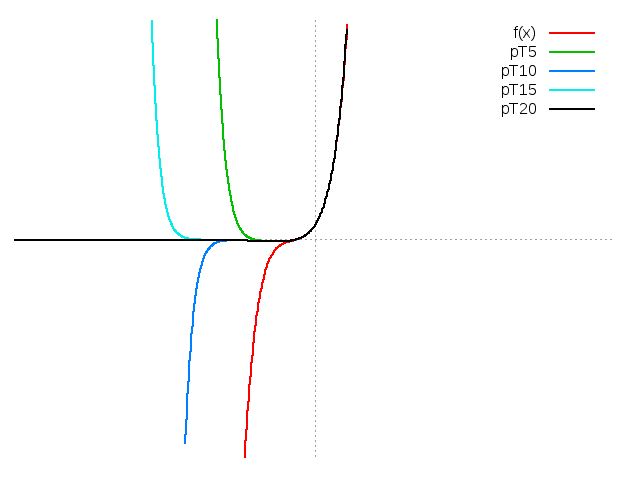
\includegraphics[scale=0.4]{1xexp}
\end{figure}
\end{tabular}


% Nunca debe faltar esta última linea.
\end{document}
